\documentclass[phd, 12pt, print]{fauthesis}
% The "print" class option overrides any special formatting of links by the hyperref package.
% Use the "online" class option instead to color links and/or put boxes around them.
%% The hyperref package embeds document data in PDF files, and automatically creates PDF bookmarks for chapters and sections.  The following lines activate it and set some of its options.
%
% NOTE: The "print" class option above will override the options used here to color the links.  Change the class option to "online" to avoid this.
%%
\usepackage{hyperref}
\usepackage{graphicx}
\usepackage{listings}             % Include the listings-package for code
\usepackage[sorting=none]{biblatex}
\addbibresource{fausamplethesis.bib}


\hypersetup{
	pdftitle={fausamplethesis},						% title
	pdfauthor={Hector Lopez},								% author
	pdfsubject={Sample file for the fauthesis document class.},	% subject of the document
	pdfnewwindow=true,								% links in new window
	pdfkeywords={FAU, thesis, dissertation, guide, TeX, LaTeX, class, style, format},		% list of keywords
	colorlinks=true,										% false: boxed links; true: colored links
	linkcolor=[rgb]{0.7,0.0,0.0},							% color of internal links
	citecolor=[rgb]{0.0,0.4,0.4},							% color of links to bibliography
	filecolor=[rgb]{0.0,0.0,0.8},							% color of file links
	urlcolor=[rgb]{0.0,0.0,0.8}								% color of external links
}


\title{A Game Theoretic Approach for Hybrid Configurations of 
Distributed Energy Resources and EV Charging Systems}
\author{Hector K. Lopez}
\gender{M}
\graduation{December}{2021}
\department{Department of Computer \& Electrical Engineering and Computre Science}
\college{Charles E.~Schmidt College of Science}
\chair{Warner A.~Miller}
\dean{Russell Ivy}
\deantitle{Interim Dean}
\dgc{Deborah L.~Floyd}[Ed.D.]

\advisor{Dr. Ali Zilouchian}
\supervisor{Andy Lau}
\supervisor{Theodora Leventouri}
\supervisor{Korey Sorge}
\signaturepush{-2.0}	% 	Increase or decrease the vertical gap between committee and administration signatures

\begin{document}
\frontmatter
\maketitle
\makecopyright
\makesignature
\begin{acknowledgements}
  To be completed later.
\end{acknowledgements}
\begin{abstract}
  To be completed later.
\end{abstract}
%\dedicate{To the graduate students of Florida Atlantic University.} 		% Optional
\tableofcontents
\nolistoftables					% Or \listoftables if there are tables
\listoffigures					% Or \nolistoffigures if there are no figures

\mainmatter

\chapter{Introduction} % Main chapter title

To be completed later.

\chapter{Background Information} % Main chapter title

\label{Chapter2} 

%----------------------------------------------------------------------------------------
%	Background Research 
%----------------------------------------------------------------------------------------

\section{Preliminary}

Game theory is a mathematical tool and conceptual framework, according to \cite{Mediwaththe}.
It is useful when studying complex, self-interested interactions among rational players. 
A simpler explanation, Game theory is the science of decision making. Game theory originated 
in the early 1940s. Economists like John Von Nuemann and Oskar Morgeston pioneered many 
of the original concepts; \textit{Theory of  Games  and  Economic  Behavior}\cite{Neumann}. Cournot, Bertrand and 
Von Stackelberg added perspectives around different types of games \cite{Azad}. It was in the 
1950's that John Nash published several ground-breaking works around special type of game involving 
compettition. John Nash introduced concepts like the Nash equilibrium and Nash bargaining, 
they where applied to competitive games and cooperative games. The latest developments came from 
John Maynard Smith (along with Ernst Mayr and G. Williams) “for developing  the  concept  of  evolutionary  biology,"
\cite{Smith1,Smith2,Smith3}. The adoption of Game theory grew because it was easy to form 
problems into the basic elements needed. Many optimization problems involve agents in some way, 
the decisions are oftengeneralized into mathematical constraints when applying traditional optimization techniques.
The complexity of these optimization problems can be reduced when modeling the agents as rational
agents with decisions to make instead of elaborate mathematical solution spaces with questionable 
edge cases to consider. 

Game theory assumes that a rational agent, also known as a \textit{player}, has its own 
cost function. The rational agent will try to optimize its own cost function, also known 
as \textit{utility},when presented with a set of options. Games in general are defined in 
\cite{McEachern} as any situation involving more than one individual. Either individual can take more 
than one action. The individuals take actions influenced by the actions of others. Finally, the 
actions taken maximize the individuals utility, also known as a \textit{pay-off}. Game theory 
defines a series of actions as a \textit{strategy}. The strategy available to an agent/player 
is like a constraint. Depending on how the game is modeled the strategy available to a player 
may be different to each player. An illustration of what strategies look like is given by \cite{Azad}, 
as a game of chess played through another person; a proxy player. If the proxy player takes 
one move in any direction the opponent will respond in many different ways. As the actual player
one must prepare a response for each of the opponents possible actions. The proxy player would 
need a set of actions to each possible response of the opponent. The set of actions that the 
proxy player would take is the strategy one has provied for the proxy player \cite{Girshick}.

\subsection{Basic Elements in a Game}

When modeling a market the players can be considered \textit{firms}. The firms would 
consider the market demand and try to minimize payments or maximize incomes. These types of  
games are usually modeled with more than one firm. Lets consider a game where there are 
\textit{n}-players \cite{Cheng}.The elements of the game can be expressed as:

$$G = [N;S_{1},S_{2},...,S_{n};u_{1},u_{2},...,u_{n}]$$ (1)

Where the game is \textit{G}, and \textit{N} represents a set of players/firms 
in the \textit{n}-player game. The \textit{S} series represents the strategies 
of each \textit{n}-player. Finally the \textit{u} represents the payment for 
each \textit{n}-player. 

\begin{enumerate}
\item \textbf{Players/Firms}: The participants in the game who can decide their own strategies.
An important assumption is that the players are rational, which means that they don’t 
leave things to chance and don’t take advantage of others’ mistakes.\cite{Mediwaththe} If the agent has perfect
rationality and all relevant information. The agent can model the game as an optimization problem. 
Unfortunately according to \cite{Mediwaththe} people do not always choose the most 
rational choice in real life.
\item \textbf{Pay-offs}: After each player in the game chooses a  strategy
from  their  own  strategies  set,  a  relevant  result  
(a  group of data) is provided to show each player’s gain or loss.
A good payoff is the fundamental goal of a player, and is the main
basis of a player’s judgment and behavior. Pay-offs are also known
as the players preferences described as 'utility' and must be 
understood clearly for the model to be effective. The payoffs are
very subjective. If there is a ranking to the payoff it is called 
\textit{ordinal} , if it is just a subjective quantity value then it is 
a \textit{cardinal} payoff.\cite{Mediwaththe}
\item \textbf{Strategy}: 
A set of available actions that can be taken by a player. In a \textit{finite game} the 
number of actions the player can pic comes from a finite set. This is similar to 
a chess board or a tic-tac-toe game, so it is also known as a \textit{matrix game}.\cite{Zhang} 
Alternatively an \textit{infinite game} set of actions means that the actions available 
to the player or on a \textit{continuous-kernel} with respect to the action variables 
of all players. In either type of action set the strategy would be the available actions as a 
space of actions available to the player.\cite{Zhang} 
\end{enumerate}

\subsection{Pay-Off Matrix}
The normal-form representation for the standard game model is 
the pay-off matrix as described by \cite{McEachern}. Each individual cell of the matrix 
typically contains comma seperated values. The first value corresponds to row and the 
second value corresponds to the column. Each row is an individual action one of the players can take.
The second player's actions are represented with each column. Since the matrix looks 
at the intersection of decisions between actions of each player the values represent 
each players pay-off for the actions corresponding with the row and column.
In \ref{fig:Pay-offMatrixfor2PlayersSample} the rows and columns are labled with actions 
$A$ and $B$ for Player 1 and Player 2. The assumption is that the players have the same 
actions available in the game, this may not always be the case. Another asumption is the 
pay-off for each player. In this example when both players choose $A$  or when both 
players choose $B$ they each have a pay-off of $0$. By analyzing this simple pay-off matrix
it is plain to see that when the players implement opposing actions they both are awarded with 
$1$. This game may represent the interaction of two agents walking into each other. The actions
can represent a simplified move to the left or right. The pay-offs would make sense in this 
example since the agents objective function would be to choose the actions that would allow them
to avoid collision and continue on thier way. 

\begin{figure}[th]
    \centering
    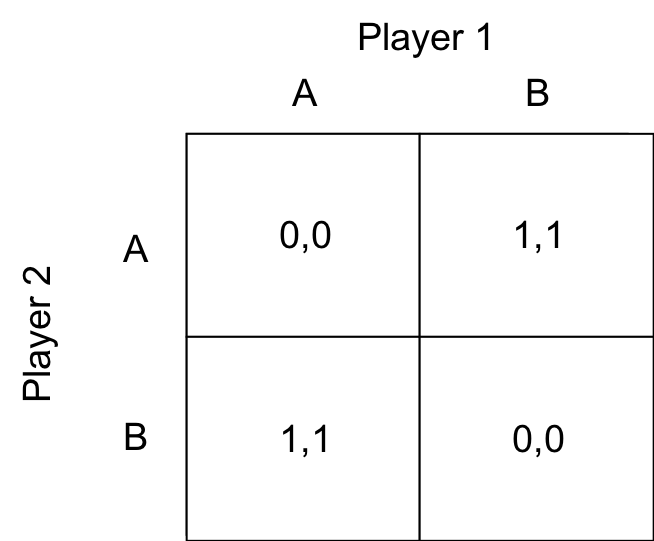
\includegraphics[width=5.0in]{Figures/pay-off-matrix-sample.png}
    \caption[A 2-Player Pay-off Matrix]{Example of a collision pay-off matrix for 2 players.}
    \label{fig:Pay-offMatrixfor2PlayersSample}
  \end{figure}

  
%\subsection{Pay-Off Matrix Example}

Let's continue with another example to illustrate the pay-off matrix and demonstrate another 
non-cooperative game. A problem to consider is an automotive intersection with a stop light. 
Both drivers can be considered as players in this game and the decisions they can take , stop or go, 
can be expressed in with the pay-off matrix. The rewards for the game can be arbitrarily 
estimated given the desire of either players. 

If both players decide to \textit{go} at the same time then they will end up in a collision. 
This does not benefit either player so we place the reward for each accordingly (pay-off of -5). 
If either of the drivers have to stop to let the other go then the player who is stopped 
is inconvenience (pay-off of 0), while the driver who was able to go is now on its way and happy (pay-off of 1). 
Finally, if both players are stopped and niether move forward  they are wasting time at the intersection.
It is not as bad as a collision but it still can be considered a loss (pay-off of -1).

\begin{figure}[th]      
  \centering
  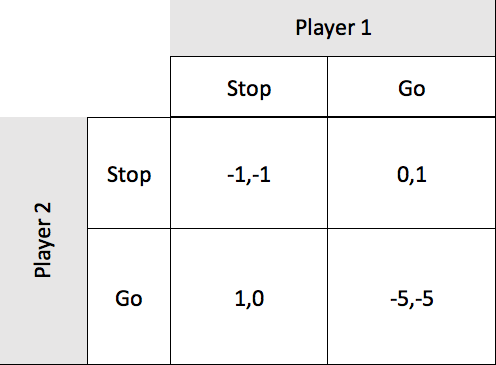
\includegraphics[width=3.0in]{Figures/pay-off-matrix.png}
  \caption[A 2-Player Pay-off Matrix]{A traffic-light pay-off matrix for 2 players.}
  \label{fig:Pay-offMatrixfor2Players}
\end{figure}


\begin{figure}[th]
  \centering
  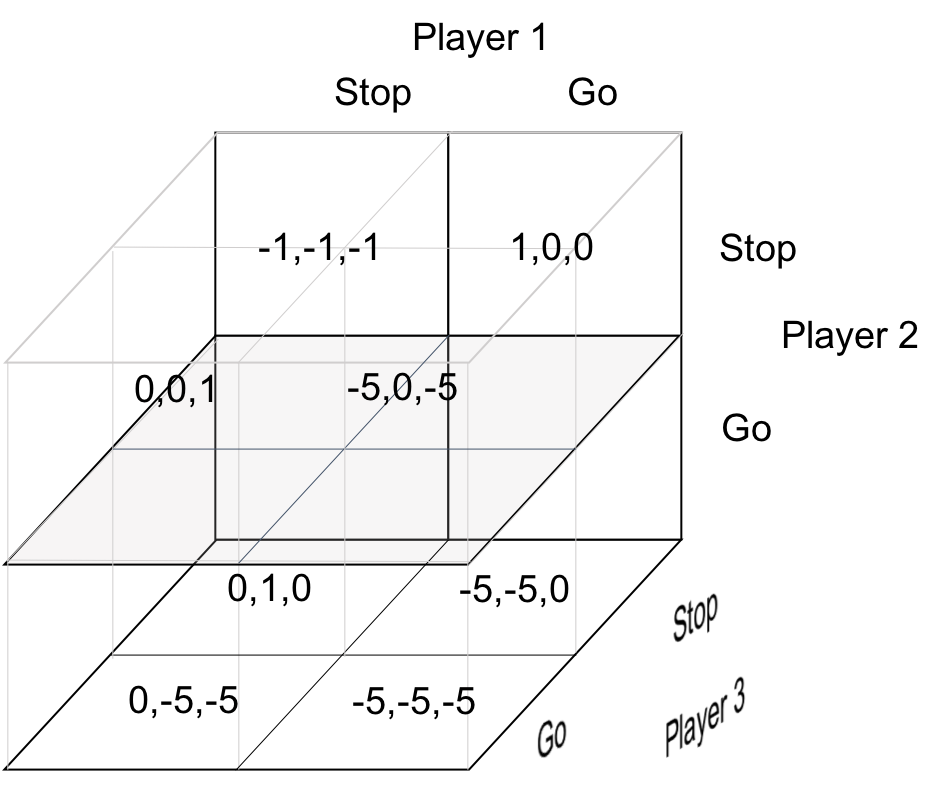
\includegraphics[width=5.0in]{Figures/3way_intersection}
  \caption[A 3-Player Pay-off Matrix]{A traffic-light pay-off matrix for 3 players.}
  \label{fig:Pay-offMatrixfor3Players}
\end{figure}


The possible decisions of the players in the game are
mapped out in the game matrix. The strategy for each player 
can now be assesed. The goal would be to find the best strategies
for player 1 and for player 2 respectively. For player 1, 
the strategy where he is able to go is when player 2 must stop
(1,0). The best strategy for player 2 is the opposite (0,1).
Since there are no better moves for each player to take these 
are both known as Nash Equilibriums. The equilibrium of a non-cooperative
game is when either player has no other decisions available that 
would better thier individual positions. There can be more than 
one nash equilibrium in a game.


\section{Cooperative Games}

Cooperative games focuses on providing incentives to independent deision makers
to act as a team to improve their position in the game. \textbf{Nash Bargaining}
is the stufy of terms and conditions where players may agree to form a coalition.
\textbf{Coalitional} gams deal with formation of coalitions.\cite{Tushar2} The coalitional
game the set of players is called a coalition and they will all have the same value
function. Coalitional games can be classified into :
\begin{enumerate}
  \item Canonical coalitional game : Study the properties and stability of the coalition, 
  the gains and the distribution of the gains in a fair manner. A solution is when all 
	players do not have an incentive to regect the revenue allocation of the coalition.

	\item Coalition formation game : The game incorporates a cost of cooperation that 
	considers the gains to the members but also the cost of forming the coalition in the 
	first place. Changes in number of players or variation of network topology can change 
	the outcome of coalitional structures.

	\item Coalitional graph game : The commnincation structures between players have an impact on the
	utility and other characteristics of the game. The main objectives is to create low-complexity
	distributed algorithms for players who wish to build a network graph and study properties
	such as stability and effeciency of the network.

\end{enumerate}



\section{Non-Cooperative Games}

In a non-cooperative game each player has control over a set of variables and strives
to optimize his individual objective function, regardless of its impact on other players.
These games allow players to take necessary action to optimize without coordination or communication. 
Even though non-cooperative game may seem like there is no cooperation involved, the term actually
refers to the lack of sharing strategic choices and communication during the game.\cite{Tushar2}
If the players obtain an equilibrium solution, it is called the \textit{Nash Equilibrium},
which is the most common concept of non-cooperative game.\cite{Azad}  In some design problems there 
are closed form expressions of the Nash equilibrium. In general numerical techniques are required
to find the solution. Some of the methods to find the Nash equilibrium provied by \cite{Azad} :

\begin{enumerate}
  \item Nikaido-Isoda function : 
  \item Rational reaction set with DOE-RSM (Design of experiment- response servce method):
  \item Monotonicity analysis:
\end{enumerate}

Lets model a  non-cooperative game as, ${\{\mathcal{N};(S_{n})_{n\in \mathcal{N}};(U_{n})_{n\in \mathcal{N}}\}}$.
Then a Nash equilibrium can be thought of as a vector of actions $\textbf{s}^{*}$ such that the 
$U_{n}(\textbf{s}^{*}) \geq U_{n}(s_{n},\textbf{s}^{*}_{-n}), \forall n \in \mathcal{N}$, 
where $s=[s_{n},\textbf{s}_{n}]$. So a Nash equilibrium can refer to the state where no player $n \in \mathcal{N}$
can improve its utility by unilaterally altering its action $s_{n}$ from $s^{*}_{n}$ 
when the actions of the other participating players are fixed
at $\textbf{s}^{*}_{-n}$. In a game where every action is deterministic (\textit{pure strategy}) 
there may not be a Nash equilibrium solution available. Also there may be more than
one Nash equilibrium in non-cooperative games. It is especially difficult 
to find the Nash equilibrium when there are more than two players. After obtaining it the 
best Nash equilibrium needs to be chosento optimize effecency if there are more than one. 
It is also important to note that a Nash equilibrium would always be present in a game where 
there is actions are probabilistic. (\textit{mixed strategy}).\cite{Tushar2}

Modeling the non-competitive game to represent the problem yeilds different models. 
There are different types of models that can be created when dealing with
non-cooperative games. By adjusting the elements of the game such as
'order' , allowing one player to go before the others, the model of the game
results in a different way to solve for the best response and resulting
equilibrium states. 

\begin{enumerate}
	\item \textbf{Ordinary Non-Cooperative game}: Analyze the problem and abstract the players,
	strategies and the pay-offs for the model. The properties of the model should 
	result in equilibrium solutions that could solve the problem.

	\item \textbf{Generalized Nash equilibrium game}: Each  player’s  decision affects 
	not only other players’ payoffs, but also their feasible strategies set.
	
	\item \textbf{Cournot game}: Derived from prisoner's dilemma model. Models the pay off  
	capable in a game when both players will need to implement the strategy at the
	same time. Used in behavioral economics to determine pay-off of individual decisions.
	
	\item \textbf{Stackelberg game}: Similar to the Cournot game, but assumes that there is a 
	player that is a leader (goes first) and a player that goes after (follower).
	The model has the leader anticipate the followers response and include that 
	in its own response. This technique helps the leader to optimize its utility
	in a market shared among two players.
	
	\item \textbf{Bounded rationality game}: Models that attempt to remove the assumption
	that players are completely rational. Considering that players can take
	actions that do not immediately benefit them can possibly model the 
	uncertainty of initial value assumptions of the utility modeled for each player.
	
	\item \textbf{Repeated game}: A series of basic games one after the other. This type of 
	model shows the varied results capable given the strategies implemented in 
	each instance of a game.
\end{enumerate}


\section{Stackelberg Oligopoly}
A Stackelberg Game is a type of noncooperative game that deals with a 
multi-level decision making process of a number of independent decision 
makers or players(followers) in response to the decisiont taken by a 
leading player (the leader).

The game has the following components:

\begin{enumerate}
	\item Followers in the game that respond to a price set by the leader
	\item The strategy of each of the followers in terms of satisfying some constraint.
	\item The utility function of each follower that captures the benefit of consuming the demand.
	\item The utility function of the leader which captures the total profit.
	\item The price per unit quantity
\end{enumerate}


\begin{figure}[th]
  \centering
  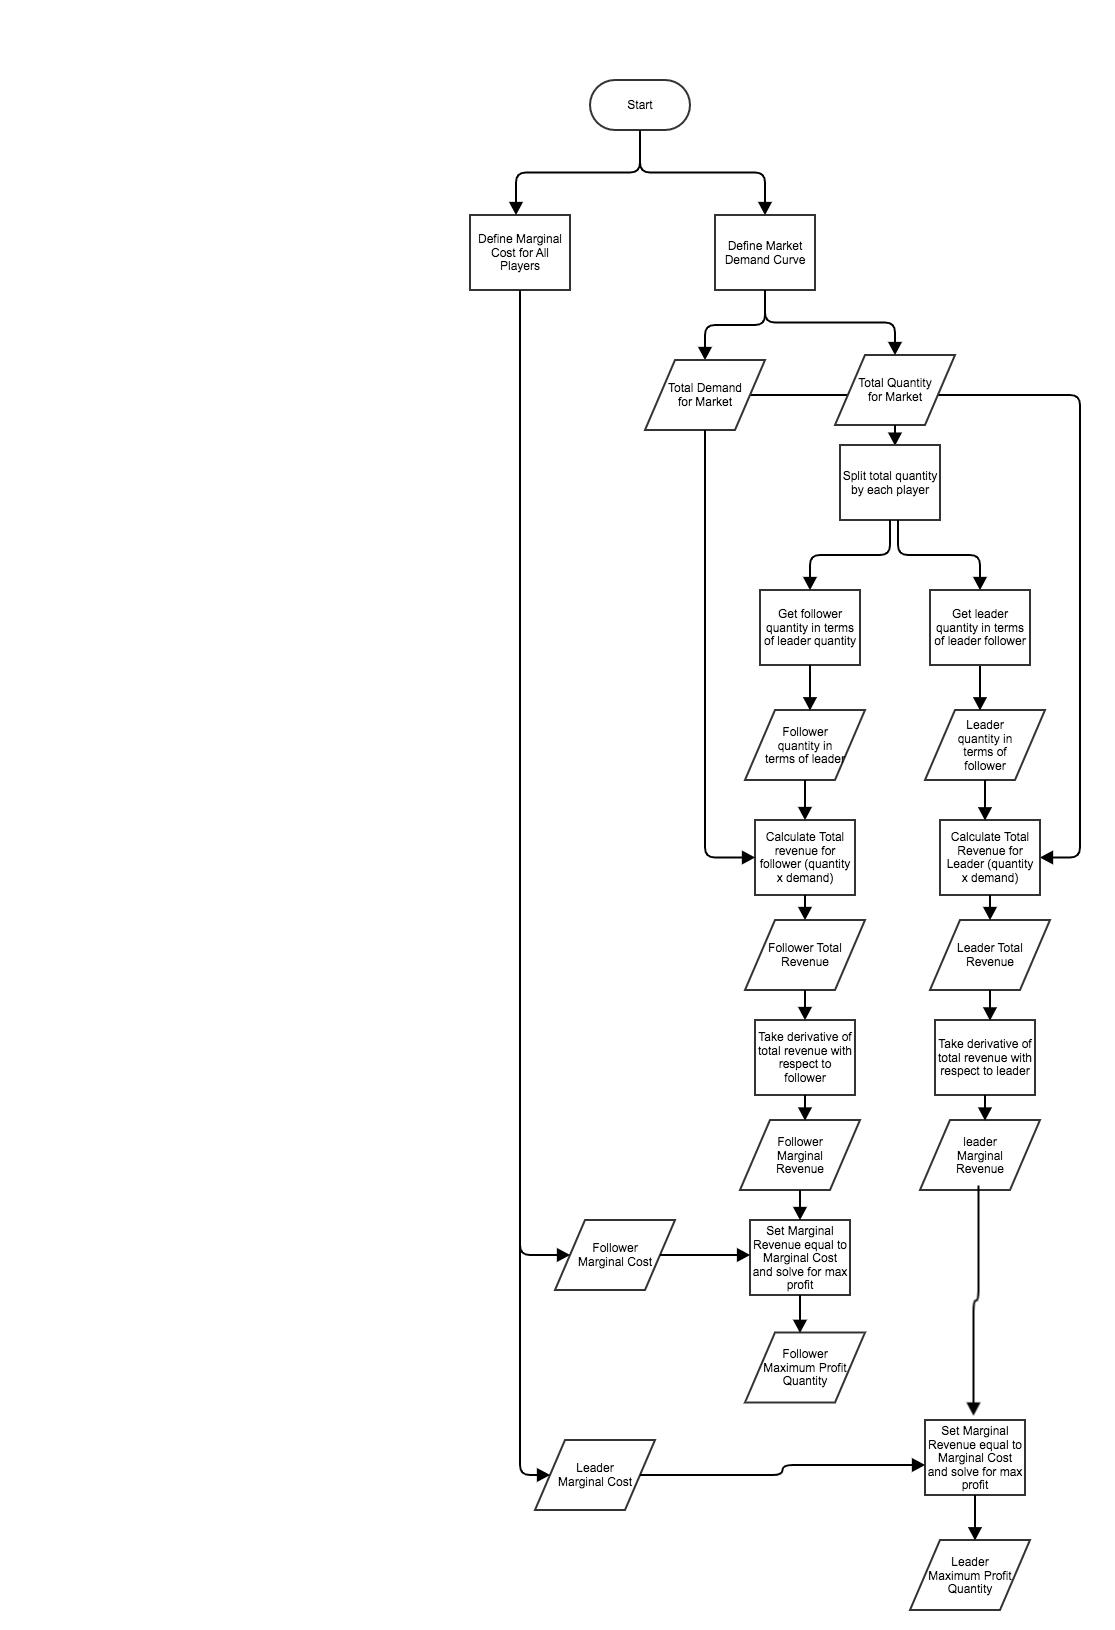
\includegraphics[width=3.5in]{Figures/stakelberggame.png}
  \caption[A Stackelberg Game Flowchart]{A flowchart showing how a backward induction 2-player Stackelberg Oligopoly game would play out.}
  \label{fig:StackelbergGame}
\end{figure}


The utility function of the follower represents the level of 
satisfaction of the follower. It is a function of the profit it recieves. 
The utility function is non-decreasing because each follower is 
interested in maximizing its profit. The marginal benefit of the 
follower is also considered a non-increasing function. The marginal 
benefit gets saturated the closer it gets to the maximum profit. 
The utility of a follower decreases as the price of a unit or cost 
of meeting a demand increases .

If the constraint is the same for all players then this gives rise to 
a noncooperative resource sharing game between the followers. A game like 
this represents a jointly convex generalized Nash equilibrium 
problem (GNDP) due to the same shared constraint. In game theory the 
coupling of the constraints has solution called the Gneralized Nash 
Equilibirum(GNE).\cite{Lefeng} 

The stackleberg duoply is a non-cooperative game between two players 
where one is a leader and the other is a follower. They are the only 
two players able to supply the needs of the market by creating some 
quantity of goods. Each player has a utility function that will be 
satisfied if they can maximize the profit of supply a quantity of 
goods to the demand curve of the market considering the cost to provide 
a unit of goods. \cite{Zhang} ,\cite{Tolwinski} 

Define a pricing demand as a linear function and call it a 
"Market Demand Curve"

$$ P = a  -  b * Q $$ (1)

Where $Q$ is the market quantity demanded and $P$ is the market price in dollars
The firms create the quantity. The terms for the curve $a$ and $b$ are constants 
set for drawing a line, where $a$ is the y-intercept and $b$ is the slope of the line.

The quantity created for the market comes from multiple firms. 
The firms in a Stackleberg game provide some quantity after the 
leader firm goes first. The leader firm assumes the moves of the 
other firms and tries to maximize its profit by incurring the costs 
to meet the demand that it deems appropriate given its own costs. 
The demand is met through a total quantity that can be represented 
by the combination of all of the players quantity. 

$$ Q = q_{1} + q_{2} + ... q_{N} $$ (2)

The cost to meet a single unit of demand per unit qunatity created. 
This is a pre-defined metric or can be a dynamic value. Knowing the 
marginal costs is critical to determining the other players moves. 
The Leader needs to know what it would cost other players to take action.

Begin backward induction to determine what the reaction would be of 
the other firms. Lets assume two firms A, and B. The procedure to 
determine the Leaders (firm A) move would be as follows:

1. Calculate Firm B's reaction
2. Calculate Firm A's response to B's reaction
3. Implement Firm A's response
4. Calculate Firm B's response given A's response
5. End Game


\subsection{2-Player Stackelberg Oligopoly Example}

$$ N_{firms} = 2$$ (3)
$$ MC_{a} = 10$$ (4)
$$ MC_{b} = 12$$ (5)
$$ P_{T} = -Q_{d}m+b$$ (6)
$$ P_{T} = -Q_{d}*0.5+120$$ (7)

To avoid having to supply diminishing returns the leader can take 
into account the maximizing move for the second player and then 
include that in determining its stake in the market based on its 
own costs and break even point.

Total Market Quantity :

$$ Q_{d}= q_{a} + q_{b}$$(8)

Begin by substituting (6) for $Q_{d}$ into the 
two quantity terms for player ${a}$ and player ${b}$ as shown in (8). 

$$ P_{T} = -0.5*q_{a} + -0.5*q_{b} + 120$$ (9)

Then replace $P_{T}$ in (8) with its definition in (7) to get the market demand
in terms of total quantity and player quantity.  

Total Market Quantity Demand :
$$ -0.5*Q_{d} + 120 = -0.5*q_{a} + -0.5*q_{b} + 120$$ (10)

The total revenue will be taken in terms of the player $b$ 
by just multiplying the market demand $P_{T}$ with just the 
quantity that will be made by $b$.

Total Revenue :

$$TR_{b} = -0.5*q_{a}*q_{b} - 0.5*q_{b}^2 + 120*q_{b}$$ (11)

Marginal revenue can be derived from the derivative of the total 
revenue equation (10), with respect to the firm.

$$ MR_{b} = \frac{\partial d}{\partial q_{b}}(-0.5*q_{a}*q_{b} - 0.5*q_{b}^2 + 120*q_{b})$$ (12)
$$ MR_{b} = -0.5*q_{a} - q_{b} + 120$$ (13)

The reaction of the follower can be estimated by the leader by 
solving when the marginal cost of the follower will equal the 
marginal revenue of the follower. Setting them equal and solving 
for the quantity in terms of the quantity provided by the leader 
firm A we get the following reactionary quantity for firm B.

$$ q_{b}^* = -0.5*q_{a} + 108$$ (14)

The leader takes into account all the reactions and creates a 
leader response to the reactions. The approach is to use back 
induction to take the forecasted reaction of the follower when 
the marginal cost is equal to the marginal revenue (profit maximizing). 
That means that the follower will stop at some break even point 
that maximizes its profits. Given that information the leader can 
take that reaction and assume it is what the follower will do. 
The assumption is used in the price demand formula. By substituting 
equation (13) into equation (9) the demand for the leader is now 
shown below in (14). Knowing the demand the total revenue and 
marginal revenue can also be inferred.

$$ P_{leader} = -0.25*q_{a} + 66$$(15)
$$ TR_{a} = -0.25*q_{a}^2 + 66*q_{a}$$ (16)
$$ MR_{a} = \frac{\partial d}{\partial q_{a}}(-0.25*q_{a}^2 + 66*q_{a})$$ (17)
$$ MR_{a} = -0.5*q_{a} + 66$$ (18)

The last step in the backwards induction for the leader is to try to 
maximize his profit by only providing a quantity where the followers 
quantity has been considered in the game. The final quantity to be 
implemented by the leader is done just as before by setting marginal 
revenue equal to marginal cost and finding quantity.

$$ q_{a}^Final = 112$$ (19)

If we implement the leaders quantity output and then recalculate 
the resulting quantity for the follower, the follower will have a 
different output than what was orginally measured by the leader 
since the leader has now taken its maximum demand.

$$ q_{b}^Final = 52$$ (20)

\subsection{3-Player Stackelberg Oligopoly Example}
Similar to a 2-play Oligopoly we can write the equation for
the total market quantity with the additional player taking a 
share of the market. 

\begin{figure}[th]
  \centering
  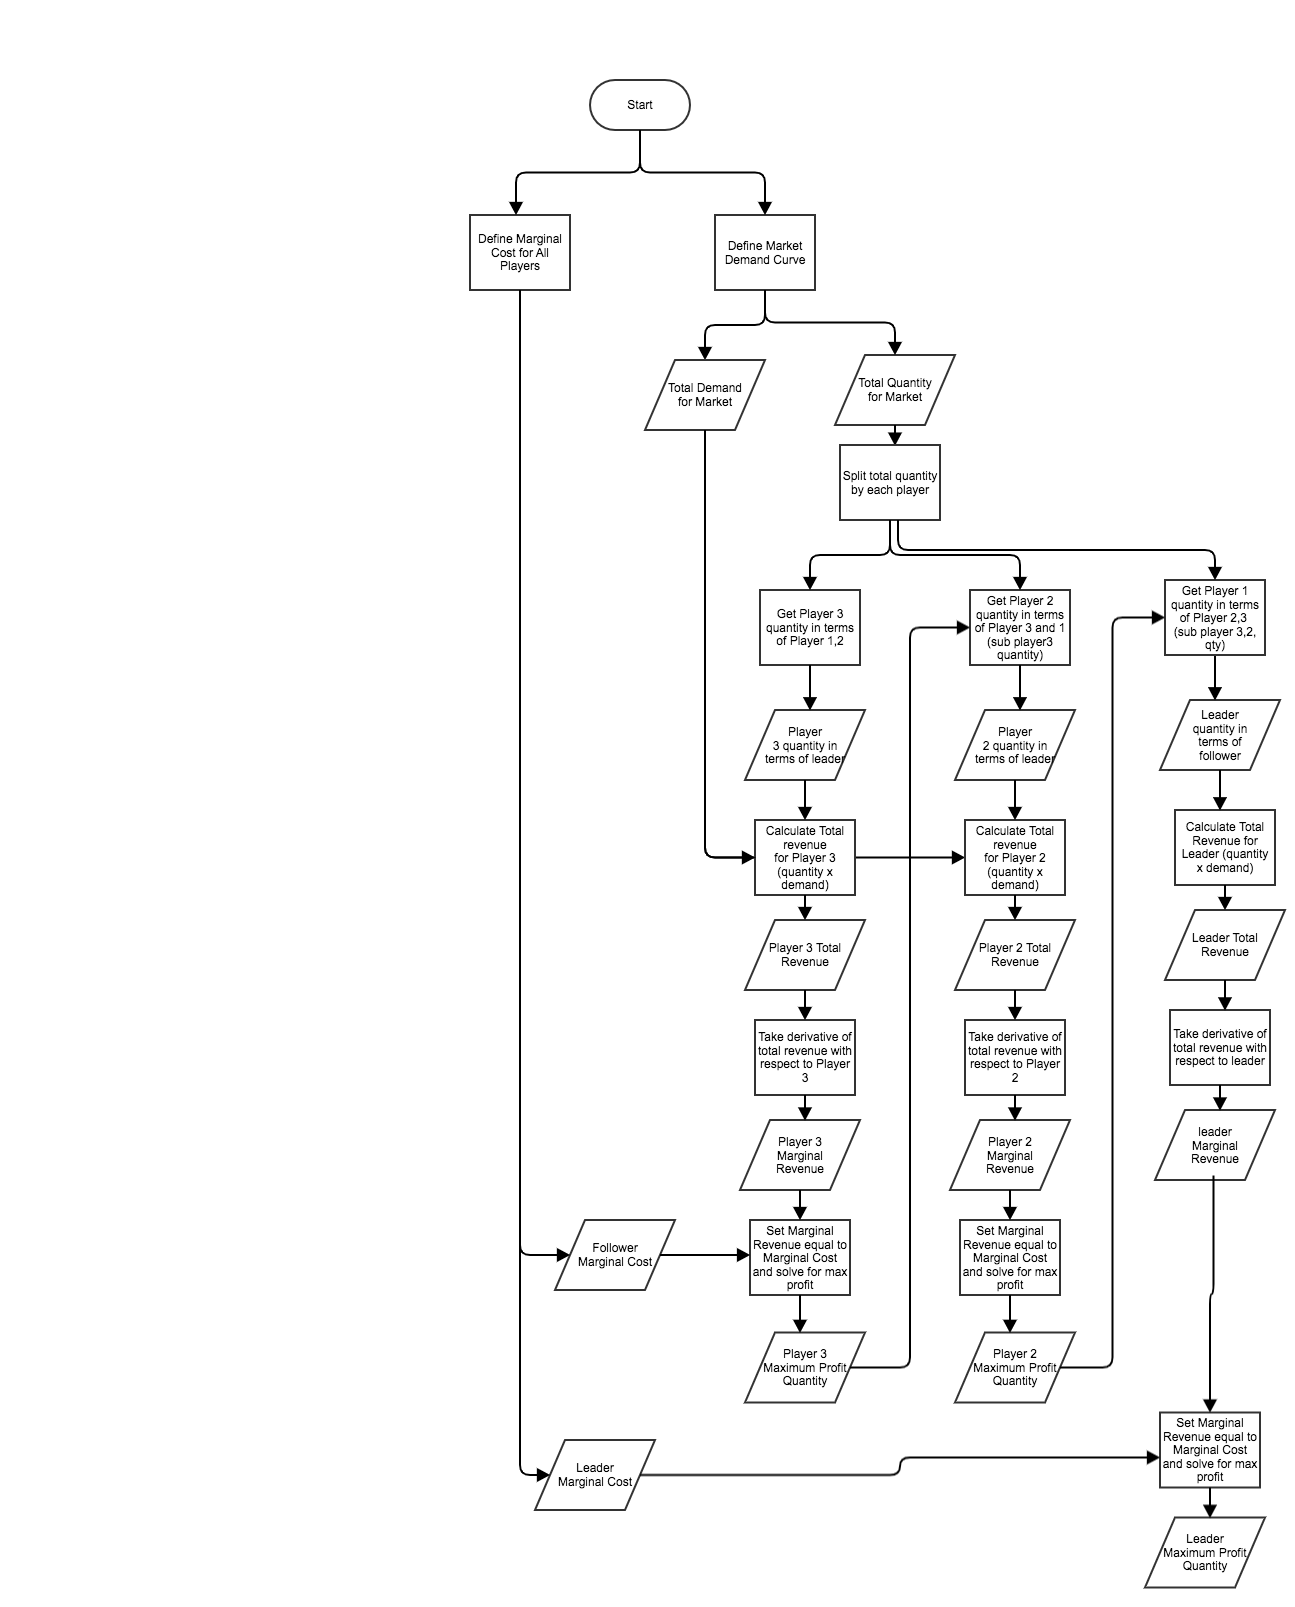
\includegraphics[width=3.5in]{Figures/stakelberggame-3pl.png}
  \caption[A Stackelberg Game Flowchart]{A flowchart showing how a backward induction 3-player Stackelberg Oligopoly game would play out.}
  \label{fig:StackelbergGame3pl}
\end{figure}


$$ N_{firms} = 3$$ (21)
$$ MC_{a} = 10$$ (22)
$$ MC_{b} = 12$$ (23)
$$ P_{T} = -Q_{d}m+b$$ (24)
$$ P_{T} = -Q_{d}*0.5+120$$ (25)


$$ Q_{d}= q_{a} + q_{b} + q_{c}$$(26)

By using the definition for market demand $P_{T}$ and the 
expanded form of the toal quantity $Q_{d}$ re-write (25) 
in terms of total quantity and quantities for each player.

$$ -0.5*Q_{d} + 120 = -0.5*q_{a}  - 0.5*q_{b} - 0.5*q_{c} + 120$$ (27)

Since backward induction forces us to begin with the last player
in order to solve this sequential game we will start by dermining the
total revenue of the last player $c$ by multiplying the 
market demand by $q_{c}$. 

Total Revenue of C: 
$$TR_{c} = -0.5*q_{a}*q_{c} - 0.5*q_{b}*q_{c} - 0.5*q_{c}^2 + 120*q_{c}$$ (28)
Marginal Revenue of C:
$$ MR_{c} = -0.5*q_{a} - 0.5*q_{b} -q_{c} + 120$$ (29)

Setting the marginal revenue equal to the marginal cost should provide the
maximum quantity required to break even for player $c$. Therefore the
best response for the last player will be in terms of what the
first and second player is a able to provide in quantity. 

Best Response for C:
$$ q_{c}^* = -0.5*q_{a} -0.5*q_{b} + 96$$ (30)

The best response for the last player is now used to calculate the best 
response for the second player. Remember that this is backwards induction
and will be used to make a decision by the leader (first player) as how
to how much it should generate in quantity. 

The same tactic as was used before to determine the Total revenue and marginal revenue
is used. Then the marginal revenue is set to the marginal cost (a constant in this case). 
The resulting maximizing value for the second player is in terms of the first and last. 
Since the last players best response has already been determined we use it in 
the best response equation for the second player. 

Best Response for B:

$$ q_{b}^* = -0.5*q_{a} -0.5*q_{c} + 98$$ (31)

Substitute 'Best Response for C' :
$$ q_{b}^* = -0.5*q_{a} -0.5*(-0.5*q_{a} -0.5*q_{b} + 96) + 98$$ (32)

Simplify Response for B:
$$ q_{b}^* = -0.375*q_{a} +0.125*q_{b} + 50$$ (33)


Now this is the last step to determine the best response for the leader.
The leader determines the total revenue amount by 
multiplying the market demand by $q_{a}$ just as it was done twice before.
Then the total revenue is used to get the marginal revenue by looking at 
the total revenue's derivative. The final step is to set it to marginal cost
and determine the maximum quantity just as it was done twice before. 
The resulting equation will be in terms of the second player and the third player.
so we substitute both players responses. 

Best Response for A:
$$ q_{a}^* = -0.5*q_{b} -0.5*q_{c} + 100$$ (34)

Substitute 'Best Response for C':

$$ q_{a}^* =  -0.375*q_{b} + 0.125*q_{a}  + 52$$ (35)

Substitute 'Best Response for B':

$$ q_{a}^* = 0.875*q_{a} + 0.046*q_{b} + 33.25$$ (36)

Simplify the Best Response for A:

$$ q_{a}^* =  (0.75*q_{a} +0.046*q_{b} + -18.75) + 0.125*q_{a}  + 52$$ (37)

\section{Game Theory Application in Energy Management}

TBD


\backmatter

\chapter{Appendix}

\section{Stackelberg Example with Python}
\lstset{language=python}          % Set your language (you can change the language for each code-block optionally)
\begin{lstlisting}[frame=single]  % Start your code-block
    from sympy import * 
    init_printing(use_latex='mathjax')
    from IPython.display import display
    import string
    alpha = list(map(chr, range(97, 123)))
    
    firms = 2
    
    N = symbols('N_{Firms}')
    display(Eq(N,firms))
    
    # Marginal Cost
    MC = [symbols('MC_%s'% i) for i in alpha]
    for i in range(firms):
        cost = 10 + i*2
        display(Eq(MC[i],cost))
        MC[i]=cost
    
    # General Market Demand Curve
    b,m = symbols('b,m')
    P_d = symbols('P_{T}')
    Q_d = symbols('Q_{D}')
    display(Eq(P_d,b-m*Q_d))
    b = 120
    m = 0.5
    display(Eq(P_d,b-m*Q_d))
    P_d=b-m*Q_d
    
    # Total Market Quantity Demand
    q = [symbols('q_%s'% i) for i in alpha]
    Q = sum(q[i] for i in range(firms))
    display(Eq(Q_d,Q))
    
    # Market Demand Curve
    P = b - m * Q
    display(Eq(P_d,P))
    
    # Total Revenue
    TR = [symbols('TR_%s'% i) for i in alpha]
    for i in range(firms-1):
        display(Eq(TR[i+1],expand(P * q[i+1])))
        TR[i+1]= expand(P * q[i+1])
    
    # Marginal Revenue
    MR = [symbols('MR_%s'% i) for i in alpha]
    for i in range(firms-1):
        display(Eq(MR[i+1],Derivative(TR[i+1],q[i+1])))
        display(Eq(MR[i+1],Derivative(TR[i+1],q[i+1]).doit()))
        MR[i+1]= Derivative(TR[i+1],q[i+1]).doit()
    
    # Reaction Functions :
    qq = [symbols('q^{*}_%s'% i) for i in alpha]
    for i in range(firms-1):
        display(Eq(qq[i+1],solve(MR[i+1] - MC[i+1],q[i+1])[0]))
        qq[i+1]=solve(MR[i+1] - MC[i+1],q[i+1])[0]
    
    # Leaders market demand in terms of leader quantity
    P_0 = P 
    P_a = symbols('P_Leader')
    for i in range(firms - 1) :
        P_0 = P_0.subs(q[i+1],qq[i+1])
    
    display(Eq(P_d,P))
    
    display(Eq(P_a,P_0))
    
    TR_0 = expand(P_0 * q[0])
    TR_a = symbols('TR_a')
    display(Eq(TR_a,TR_0))
    
    MR_0 = Derivative(TR_0,q[0]).doit()
    MR_a = symbols('MR_a')
    display(Eq(MR_a,Derivative(TR_0,q[0])))
    display(Eq(MR_a,MR_0))
    
    # Most profit maximizing quantity for leader is q_0
    q_0 = solve(MR_0-MC[0],q[0])[0]
    q_a = symbols('q^Final_a')
    display(Eq(q_a,q_0))
    
    # Reactions Taken :
    qqq = [symbols('q_%s__Final'% i) for i in alpha]
    for i in range(firms-1):
        display(Eq(qqq[i+1],qq[i+1].subs(q[0],q_0)))
        qqq[i]=qq[i+1].subs(q[0],q_0)
    P_d=b-m*Q_d
    display(Eq(Q_d,Q))
    q[0] = q_0
    for i in range(firms-1):
        q[i+1] = qqq[i]

\end{lstlisting}



\printbibliography

\end{document}